% Engineering Methods

\documentclass[10pt ,english,a4paper]{article}

\usepackage[english]{babel}
\usepackage[IL2]{fontenc}
\usepackage[utf8]{inputenc}
\usepackage{graphicx}
\usepackage{url}
\usepackage{hyperref}
\usepackage{times}

\pagestyle{headings}

\title{Use of artificial intelligence in a field of obtaining information from documents using probabilistic model\thanks{Semestral project in subject Engineering Methods, ac. year 2023/24, guidance: MSc. Mirwais Ahmadzai}}

\author{Alžbeta Žiarovská\\[2pt]
	{\small Slovak University of Technology in Bratislava}\\
	{\small Faculty of Informatics and Information Technologies}\\
	{\small \texttt{xziarovska@stuba.sk}}
	}

\date{\small 26. september 2023}



\begin{document}

\maketitle
\newpage

\begin{abstract}
\ldots
\end{abstract}
\newpage

\section{Introduction}

This article concludes creations of many scientists and researchers who were all devoted to finding out as much as possible in a field of information retrieval. "Information retrieval" is a enormously broad term. I would like to work with a focus on document retrieval, meaning, extracting information from documents written using natural language. 

There are many methods, which we can use to retrieve information, which will be closer addressed in subsection "Other types of models" of section "Models"~\ref{models:other} However, the main focus of this article is going to be probabilistic model, which is more deeply explained in subsection "Probabilistic model" of section "Models"~\ref{models:prob}.

Artificial intelligence has become everyday part of lives of many people. We are using a great variety of tools to help us find appropriate information we can use for numerous purposes (e.g. education, medicine,...) and, apparently, we are getting lazier by doing so. \cite{ahmad23impact}
	

\paragraph{Spoločenské súvisloti}

Toto je paragraf, neviem, ako sa ukáže, to idem teraz zistiť, aka fuka funda luka... Čo sa stane? Rozbijem to?
Pokračujem v Introduction, alebo? Možno ani nepokračujem \cite{jones99info}a možno pokračujem.

\section{Information retrieval from documents}\label{ir}

Information retrieval from documents (further in article I will refer to this term only as document retrieval) is a main term of this paper. It is referring to a primarily linguistic process of extracting information from textual material or documents. The least we have to do in this process is to describe want we are yearning for and make this description compatible with descriptions of information we have access to. Furthermore, our description of what we are looking for must have a meaning. \cite{blair03info}

\section{Models of Information Retrieval} \label{models}

By using terminology an information retrieval system (model) we understand a software algorithm which stores and manages information obtained from documents (often textual, but multimedia is also a possibility). The purpose of the system is to assist a user in finding the exact information they are looking for and need. The system does not explicitly answer questions or return information. However, it offers a information that contains existence and location of documents which might possibly hold the information desired by the user. The main goal is to satisfy user's need of information and some of the found documents will hopefully achieve user's satisfaction. The documents that fulfill this goal are called \emph{relevant documents}. A retrieval system that is perfect would only retrieve documents that are relevant and no irrelevant documents would be offered. Nevertheless, such system does not exist and will never exist either, mostly because relevance is a subjective opinion of the user.

We distinguish three primal processes an information retrieval system has to be able to provide:
\begin{enumerate}
\item The representation of the content of the documents
\item The representation of the user's information need
\item The comparison of the two representations
\end{enumerate}

These processes are shown in the Figure \ref{f:process}. In the figure, blue colored boxes represent processed and red colored boxes represent data.

\emph{Indexing} usually refers to process of representing the documents. The process happens off-line, meaning, there is no direct involvement of the end user of the information retrieval system. The result of the indexing process is a representation of the document. Documents are often only stored partially, for example only the title and the abstract, plus the actual location of the document. However the indexing might include the actual storage of the document.

The process of representing the user's \emph{need for information} if often called the \emph{query formulation process}. In general, query formulation may denote the complete interactive dialogue between user and system. This leads not to only accurate query but possibly also to bettering user's understanding of their information needs. This part is visualized by the feedback process in Figure \ref{f:process}.

The comparison of the query against the document representations is referred to as \emph{matching process}. The process ordinarily results in a ranked list of documents. User is able to go through the list and search for the information they need. To minimize the time user needs to find the information, ranked retrieval hopefully puts the relevant documents on the top of the list. Effective ranking algorithms are rather simple, they use frequency distribution of terms over documents as well as statistics over other information. Effective ranking algorithms might easily halve the time user spends on reading documents. \cite{hiem09info}

\begin{figure*}[tbh]
\centering
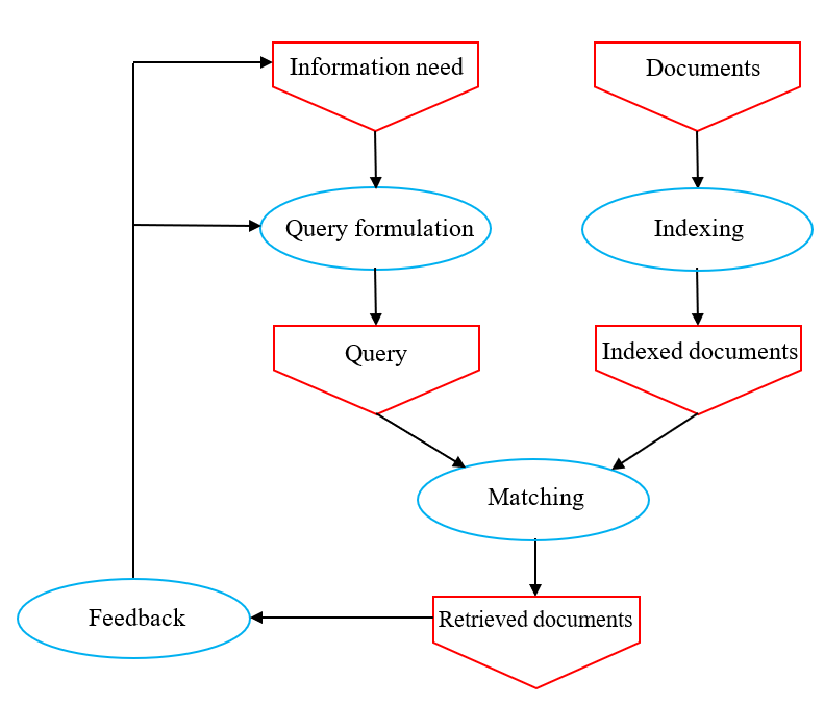
\includegraphics[scale=0.75]{figure1.pdf}
\caption{Information Retrieval Processes}
\label{f:process}
\end{figure*}

\subsection{Probabilistic model} \label{models:prob}
\cite{hiem09info}
\cite{jones99info}

\subsection{Other types of models} \label{models:other}

There will be two information retrieval models mentioned and addressed in this section. Both of them provide exact matching (documents are either retrieved or not), but there is no ranking of the retrieved documents.

\paragraph{The Boolean model} 

The Boolean model is believed to be the first information retrieval model and probably is also one of the most criticized ones. It can be explained by defining query as a unambiguous definition of a set of written documents. To give an example the query term economic defines the group of all documents that are indexed with the label economic. New sets of documents can be creating by combining query terms and their competent sets of documents using the operators of Boole's mathematical logic.

The main advantage of this type of IR model is giving a sense of control over the system to the user. A user can be certain, why has the document been retrieved. According to the document sets' size it is immediately clear which operators of Boolean algebra (AND, OR, NOT) will produce a smaller or bigger set of documents. We can see a visualized example in a Figure \ref{f:boole}\cite{hiem09info}

\begin{figure*}[tbh]
\centering
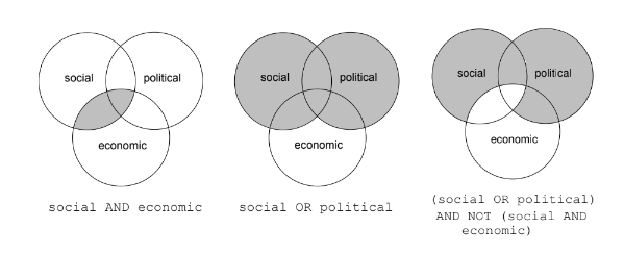
\includegraphics[scale=1.0]{figure2.pdf}
\caption{Visualization of Boolean combinations of sets by Venn diagrams}
\label{f:boole}
\end{figure*}

\paragraph{The vector space model}
The main point of approach by vector space model is to model information retrieval objects as elements of vector space. To be more specific, terms, documents, queries and so on are all vectors in the vector space. By having the vector space we have a system with linear properties, for example the ability to add together two elements to get a new one or the ability to multiply a vector by a real number.The similarity between documents and queries can be measured using these properties, such as the scalar product of the corresponding vectors. 

In a vector space model, the key components are:
\begin{itemize}
\item \emph{Dimension}: The number of terms and keywords that determines the size of the vectors representing documents and queries.
\item \emph{Basis Vectors}: A set of vectors that form a basis from the vector space. In some cases, these basis vectors may be assumed to be pairwise orthogonal, although this is not always realistic.
\item \emph{Correlations}: If the term vectors are not orthogonal, their correlations can be used to represent the relationships between terms.
\item \emph{Document vectors}: These vectors represent the documents in the vector space. The components of these vectors correspond to the weights of the terms within the documents.
\item \emph{Query vectors}: Represent the user queries, their components correspond to the weights of the terms in the queries.
\item \emph{Similarity measurement}: A method of determining the similarity between two vectors, such as the scalar product. This similarity can be used to rank documents in the order of their estimated usefulness to a user.
\end{itemize}
\cite{rag86vector}

\section{Conclusion}\label{conclusion}

Z obr.~\ref{f:rozhod} je všetko jasné. 

\begin{figure*}[tbh]
\centering
%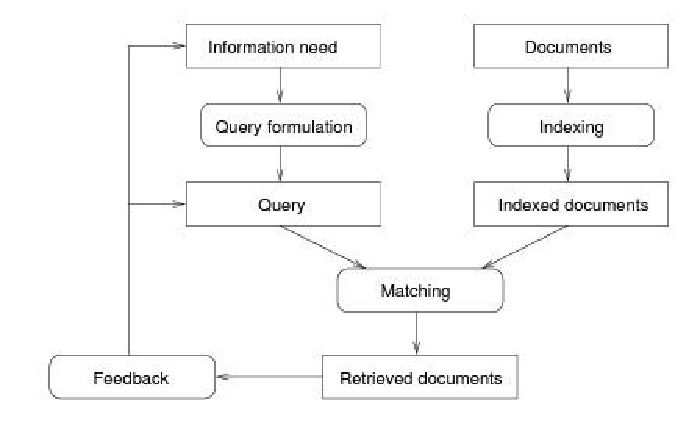
\includegraphics[scale=1.0]{irprocess.pdf}
Aj text môže byť prezentovaný ako obrázok. Stane sa z neho označný plávajúci objekt. Po vytvorení diagramu zrušte znak \texttt{\%} pred príkazom \verb|\includegraphics| označte tento riadok ako komentár (tiež pomocou znaku \texttt{\%}).
\caption{Rozhodujuci argument.}
\label{f:rozhod}
\end{figure*}



\section{Iná časť} \label{ina}

Základným problémom je teda\ldots{} Najprv sa pozrieme na nejaké vysvetlenie (časť~\ref{ina:nejake}), a potom na ešte nejaké (časť~\ref{ina:nejake}).\footnote{Niekedy môžete potrebovať aj poznámku pod čiarou.}

Môže sa zdať, že problém vlastne nejestvuje\cite{Coplien:MPD}, ale bolo dokázané, že to tak nie je~\cite{Czarnecki:Staged, Czarnecki:Progress}. Napriek tomu, aj dnes na webe narazíme na všelijaké pochybné názory\cite{PLP-Framework}. Dôležité veci možno \emph{zdôrazniť kurzívou}.

\section{Ďaľšia časť}
Toto je ďalšia časť, v ktorej idem urobiť odsek.

Toto je odsek. haha.

\subsection{Nejaké vysvetlenie} \label{ina:nejake}

Niekedy treba uviesť zoznam:

\begin{itemize}
\item jedna vec
\item druhá vec
	\begin{itemize}
	\item x
	\item y
	\end{itemize}
\end{itemize}

Ten istý zoznam, len číslovaný:

\begin{enumerate}
\item jedna vec
\item druhá vec
	\begin{enumerate}
	\item x
	\item y
	\end{enumerate}
\end{enumerate}


\subsection{Ešte nejaké vysvetlenie} \label{ina:este}

\paragraph{Veľmi dôležitá poznámka.}
Niekedy je potrebné nadpisom označiť odsek. Text pokračuje hneď za nadpisom.



\section{Dôležitá časť} \label{dolezita}




\section{Ešte dôležitejšia časť} \label{dolezitejsia}




\section{Záver} \label{zaver} % prípadne iný variant názvu



%\acknowledgement{Ak niekomu chcete poďakovať\ldots}


% týmto sa generuje zoznam literatúry z obsahu súboru literatura.bib podľa toho, na čo sa v článku odkazujete
\bibliography{literatura}
\bibliographystyle{alpha} % prípadne alpha, abbrv alebo hociktorý iný
\end{document}
